\begin{figure}
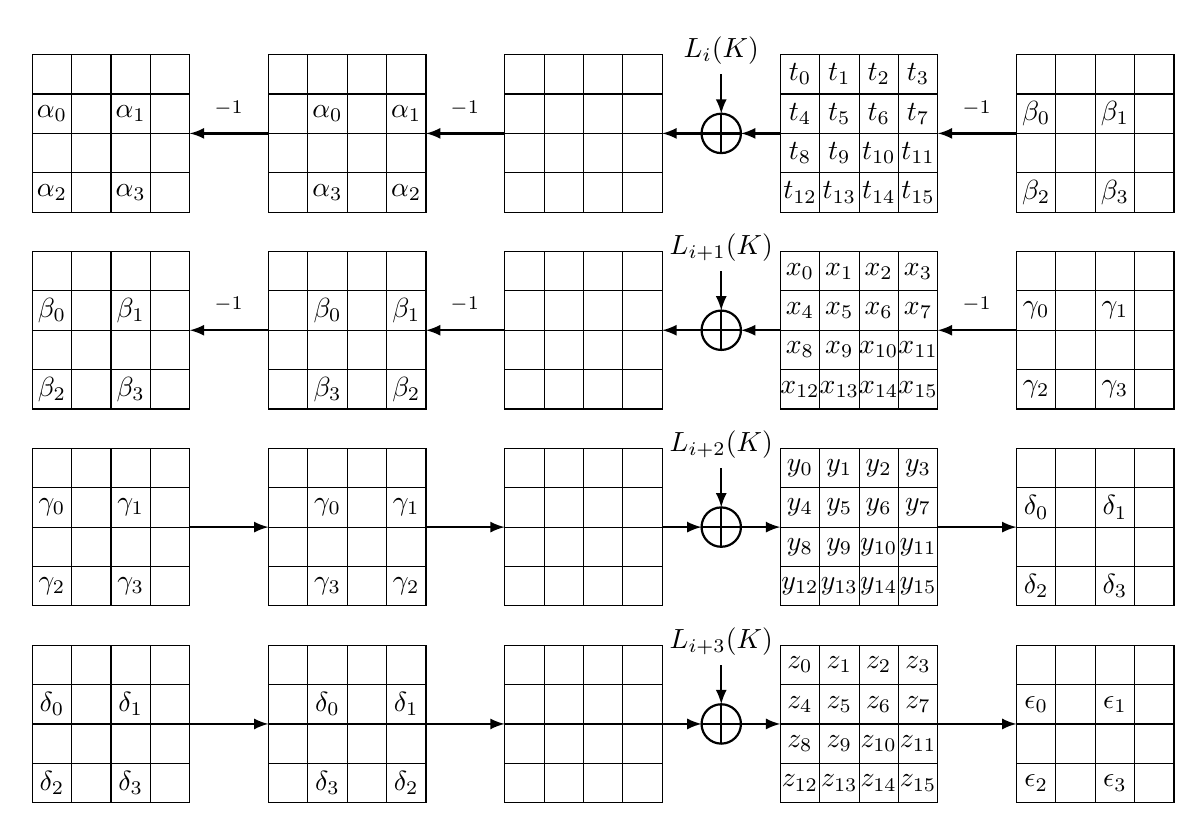
\begin{tikzpicture}[scale=.5]
%first line
\draw (0,15) rectangle (4,19);
\draw (0,16) -- (4,16);
\draw (0,17) -- (4,17);
\draw (0,18) -- (4,18);
\draw (1,15) -- (1,19);
\draw (2,15) -- (2,19);
\draw (3,15) -- (3,19);
\draw (.5,17.5) node {$\alpha_0$};
\draw (2.5,17.5) node {$\alpha_1$};
\draw (.5,15.5) node {$\alpha_2$};
\draw (2.5,15.5) node {$\alpha_3$};

\draw[<-,>=latex, thick] (4,17) -- node[above,midway] {$\shiftR^{-1}$} (6,17);
\draw (6,15) rectangle (10,19);
\draw (6,16) -- (10,16);
\draw (6,17) -- (10,17);
\draw (6,18) -- (10,18);
\draw (7,15) -- (7,19);
\draw (8,15) -- (8,19);
\draw (9,15) -- (9,19);
\draw (7.5,17.5) node {$\alpha_0$};
\draw (9.5,17.5) node {$\alpha_1$};
\draw (7.5,15.5) node {$\alpha_3$};
\draw (9.5,15.5) node {$\alpha_2$};

\draw[<-,>=latex, thick] (10,17) -- node[above,midway] {$\mixC^{-1}$} (12,17);
\draw (12,15) rectangle (16,19);
\draw (12,16) -- (16,16);
\draw (12,17) -- (16,17);
\draw (12,18) -- (16,18);
\draw (13,15) -- (13,19);
\draw (14,15) -- (14,19);
\draw (15,15) -- (15,19);

\draw[<-,>=latex,thick] (16,17) -- (17,17);
\draw[thick] (17.5,17) circle (.5);
\draw[thick] (17,17) -- (18,17);
\draw[thick] (17.5,16.5) -- (17.5,17.5);
\draw[<-,>=latex,thick] (17.5,17.5) -- (17.5,18.5);
\draw (17.5,18.5) node[above] {$L_i(K)$};
\draw[<-,>=latex,thick] (18,17) -- (19,17);
\draw (19,15) rectangle (23,19);
\draw (19,16) -- (23,16);
\draw (19,17) -- (23,17);
\draw (19,18) -- (23,18);
\draw (20,15) -- (20,19);
\draw (21,15) -- (21,19);
\draw (22,15) -- (22,19);
\draw (19.5,18.5) node {$t_0$};
\draw (20.5,18.5) node {$t_1$};
\draw (21.5,18.5) node {$t_2$};
\draw (22.5,18.5) node {$t_3$};

\draw (19.5,17.5) node {$t_4$};
\draw (20.5,17.5) node {$t_5$};
\draw (21.5,17.5) node {$t_6$};
\draw (22.5,17.5) node {$t_7$};

\draw (19.5,16.5) node {$t_8$};
\draw (20.5,16.5) node {$t_9$};
\draw (21.5,16.5) node {$t_{10}$};
\draw (22.5,16.5) node {$t_{11}$};

\draw (19.5,15.5) node {$t_{12}$};
\draw (20.5,15.5) node {$t_{13}$};
\draw (21.5,15.5) node {$t_{14}$};
\draw (22.5,15.5) node {$t_{15}$};

\draw[<-,>=latex, thick] (23,17) -- node[above,midway] {$\subW^{-1}$} (25,17);
\draw (25,15) rectangle (29,19);
\draw (25,16) -- (29,16);
\draw (25,17) -- (29,17);
\draw (25,18) -- (29,18);
\draw (26,15) -- (26,19);
\draw (27,15) -- (27,19);
\draw (28,15) -- (28,19);
\draw (25.5,17.5) node {$\beta_0$};
\draw (27.5,17.5) node {$\beta_1$};
\draw (25.5,15.5) node {$\beta_2$};
\draw (27.5,15.5) node {$\beta_3$};

%second line
\draw (0,10) rectangle (4,14);
\draw (0,11) -- (4,11);
\draw (0,12) -- (4,12);
\draw (0,13) -- (4,13);
\draw (1,10) -- (1,14);
\draw (2,10) -- (2,14);
\draw (3,10) -- (3,14);
\draw (.5,12.5) node {$\beta_0$};
\draw (2.5,12.5) node {$\beta_1$};
\draw (.5,10.5) node {$\beta_2$};
\draw (2.5,10.5) node {$\beta_3$};

\draw[<-,>=latex, thick] (4,12) -- node[above,midway] {$\shiftR^{-1}$} (6,12);
\draw (6,10) rectangle (10,14);
\draw (6,11) -- (10,11);
\draw (6,12) -- (10,12);
\draw (6,13) -- (10,13);
\draw (7,10) -- (7,14);
\draw (8,10) -- (8,14);
\draw (9,10) -- (9,14);
\draw (7.5,12.5) node {$\beta_0$};
\draw (9.5,12.5) node {$\beta_1$};
\draw (7.5,10.5) node {$\beta_3$};
\draw (9.5,10.5) node {$\beta_2$};

\draw[<-,>=latex, thick] (10,12) -- node[above,midway] {$\mixC^{-1}$} (12,12);
\draw (12,10) rectangle (16,14);
\draw (12,11) -- (16,11);
\draw (12,12) -- (16,12);
\draw (12,13) -- (16,13);
\draw (13,10) -- (13,14);
\draw (14,10) -- (14,14);
\draw (15,10) -- (15,14);

\draw[<-,>=latex,thick] (16,12) -- (17,12);
\draw[thick] (17.5,12) circle (.5);
\draw[thick] (17,12) -- (18,12);
\draw[thick] (17.5,11.5) -- (17.5,12.5);
\draw[<-,>=latex,thick] (17.5,12.5) -- (17.5,13.5);
\draw (17.5,13.5) node[above] {$L_{i+1}(K)$};
\draw[<-,>=latex,thick] (18,12) -- (19,12);
\draw (19,10) rectangle (23,14);
\draw (19,11) -- (23,11);
\draw (19,12) -- (23,12);
\draw (19,13) -- (23,13);
\draw (20,10) -- (20,14);
\draw (21,10) -- (21,14);
\draw (22,10) -- (22,14);
\draw (19.5,13.5) node {$x_0$};
\draw (20.5,13.5) node {$x_1$};
\draw (21.5,13.5) node {$x_2$};
\draw (22.5,13.5) node {$x_3$};

\draw (19.5,12.5) node {$x_4$};
\draw (20.5,12.5) node {$x_5$};
\draw (21.5,12.5) node {$x_6$};
\draw (22.5,12.5) node {$x_7$};

\draw (19.5,11.5) node {$x_8$};
\draw (20.5,11.5) node {$x_9$};
\draw (21.5,11.5) node {$x_{10}$};
\draw (22.5,11.5) node {$x_{11}$};

\draw (19.5,10.5) node {$x_{12}$};
\draw (20.5,10.5) node {$x_{13}$};
\draw (21.5,10.5) node {$x_{14}$};
\draw (22.5,10.5) node {$x_{15}$};

\draw[<-,>=latex, thick] (23,12) -- node[above,midway] {$\subW^{-1}$} (25,12);
\draw (25,10) rectangle (29,14);
\draw (25,11) -- (29,11);
\draw (25,12) -- (29,12);
\draw (25,13) -- (29,13);
\draw (26,10) -- (26,14);
\draw (27,10) -- (27,14);
\draw (28,10) -- (28,14);
\draw (25.5,12.5) node {$\gamma_0$};
\draw (27.5,12.5) node {$\gamma_1$};
\draw (25.5,10.5) node {$\gamma_2$};
\draw (27.5,10.5) node {$\gamma_3$};


%third line
\draw (0,5) rectangle (4,9);
\draw (0,6) -- (4,6);
\draw (0,7) -- (4,7);
\draw (0,8) -- (4,8);
\draw (1,5) -- (1,9);
\draw (2,5) -- (2,9);
\draw (3,5) -- (3,9);
\draw (.5,7.5) node {$\gamma_0$};
\draw (2.5,7.5) node {$\gamma_1$};
\draw (.5,5.5) node {$\gamma_2$};
\draw (2.5,5.5) node {$\gamma_3$};

\draw[->,>=latex, thick] (4,7) -- node[above,midway] {$\shiftR$} (6,7);
\draw (6,5) rectangle (10,9);
\draw (6,6) -- (10,6);
\draw (6,7) -- (10,7);
\draw (6,8) -- (10,8);
\draw (7,5) -- (7,9);
\draw (8,5) -- (8,9);
\draw (9,5) -- (9,9);
\draw (7.5,7.5) node {$\gamma_0$};
\draw (9.5,7.5) node {$\gamma_1$};
\draw (7.5,5.5) node {$\gamma_3$};
\draw (9.5,5.5) node {$\gamma_2$};

\draw[->,>=latex, thick] (10,7) -- node[above,midway] {$\mixC$} (12,7);
\draw (12,5) rectangle (16,9);
\draw (12,6) -- (16,6);
\draw (12,7) -- (16,7);
\draw (12,8) -- (16,8);
\draw (13,5) -- (13,9);
\draw (14,5) -- (14,9);
\draw (15,5) -- (15,9);

\draw[->,>=latex,thick] (16,7) -- (17,7);
\draw[thick] (17.5,7) circle (.5);
\draw[thick] (17,7) -- (18,7);
\draw[thick] (17.5,6.5) -- (17.5,7.5);
\draw[<-,>=latex,thick] (17.5,7.5) -- (17.5,8.5);
\draw (17.5,8.5) node[above] {$L_{i+2}(K)$};
\draw[->,>=latex,thick] (18,7) -- (19,7);
\draw (19,5) rectangle (23,9);
\draw (19,6) -- (23,6);
\draw (19,7) -- (23,7);
\draw (19,8) -- (23,8);
\draw (20,5) -- (20,9);
\draw (21,5) -- (21,9);
\draw (22,5) -- (22,9);
\draw (19.5,8.5) node {$y_0$};
\draw (20.5,8.5) node {$y_1$};
\draw (21.5,8.5) node {$y_2$};
\draw (22.5,8.5) node {$y_3$};

\draw (19.5,7.5) node {$y_4$};
\draw (20.5,7.5) node {$y_5$};
\draw (21.5,7.5) node {$y_6$};
\draw (22.5,7.5) node {$y_7$};

\draw (19.5,6.5) node {$y_8$};
\draw (20.5,6.5) node {$y_9$};
\draw (21.5,6.5) node {$y_{10}$};
\draw (22.5,6.5) node {$y_{11}$};

\draw (19.5,5.5) node {$y_{12}$};
\draw (20.5,5.5) node {$y_{13}$};
\draw (21.5,5.5) node {$y_{14}$};
\draw (22.5,5.5) node {$y_{15}$};

\draw[->,>=latex, thick] (23,7) -- node[above,midway] {$\subW$} (25,7);
\draw (25,5) rectangle (29,9);
\draw (25,6) -- (29,6);
\draw (25,7) -- (29,7);
\draw (25,8) -- (29,8);
\draw (26,5) -- (26,9);
\draw (27,5) -- (27,9);
\draw (28,5) -- (28,9);
\draw (25.5,7.5) node {$\delta_0$};
\draw (27.5,7.5) node {$\delta_1$};
\draw (25.5,5.5) node {$\delta_2$};
\draw (27.5,5.5) node {$\delta_3$};

%fourth line
\draw (0,0) rectangle (4,4);
\draw (0,1) -- (4,1);
\draw (0,2) -- (4,2);
\draw (0,3) -- (4,3);
\draw (1,0) -- (1,4);
\draw (2,0) -- (2,4);
\draw (3,0) -- (3,4);
\draw (.5,2.5) node {$\delta_0$};
\draw (2.5,2.5) node {$\delta_1$};
\draw (.5,0.5) node {$\delta_2$};
\draw (2.5,0.5) node {$\delta_3$};

\draw[->,>=latex, thick] (4,2) -- node[above,midway] {$\shiftR$} (6,2);
\draw (6,0) rectangle (10,4);
\draw (6,1) -- (10,1);
\draw (6,2) -- (10,2);
\draw (6,3) -- (10,3);
\draw (7,0) -- (7,4);
\draw (8,0) -- (8,4);
\draw (9,0) -- (9,4);
\draw (7.5,2.5) node {$\delta_0$};
\draw (9.5,2.5) node {$\delta_1$};
\draw (7.5,0.5) node {$\delta_3$};
\draw (9.5,0.5) node {$\delta_2$};

\draw[->,>=latex, thick] (10,2) -- node[above,midway] {$\mixC$} (12,2);
\draw (12,0) rectangle (16,4);
\draw (12,1) -- (16,1);
\draw (12,2) -- (16,2);
\draw (12,3) -- (16,3);
\draw (13,0) -- (13,4);
\draw (14,0) -- (14,4);
\draw (15,0) -- (15,4);

\draw[->,>=latex,thick] (16,2) -- (17,2);
\draw[thick] (17.5,2) circle (.5);
\draw[thick] (17,2) -- (18,2);
\draw[thick] (17.5,1.5) -- (17.5,2.5);
\draw[<-,>=latex,thick] (17.5,2.5) -- (17.5,3.5);
\draw (17.5,3.5) node[above] {$L_{i+3}(K)$};
\draw[->,>=latex,thick] (18,2) -- (19,2);
\draw (19,0) rectangle (23,4);
\draw (19,1) -- (23,1);
\draw (19,2) -- (23,2);
\draw (19,3) -- (23,3);
\draw (20,0) -- (20,4);
\draw (21,0) -- (21,4);
\draw (22,0) -- (22,4);
\draw (19.5,3.5) node {$z_0$};
\draw (20.5,3.5) node {$z_1$};
\draw (21.5,3.5) node {$z_2$};
\draw (22.5,3.5) node {$z_3$};

\draw (19.5,2.5) node {$z_4$};
\draw (20.5,2.5) node {$z_5$};
\draw (21.5,2.5) node {$z_6$};
\draw (22.5,2.5) node {$z_7$};

\draw (19.5,1.5) node {$z_8$};
\draw (20.5,1.5) node {$z_9$};
\draw (21.5,1.5) node {$z_{10}$};
\draw (22.5,1.5) node {$z_{11}$};

\draw (19.5,0.5) node {$z_{12}$};
\draw (20.5,0.5) node {$z_{13}$};
\draw (21.5,0.5) node {$z_{14}$};
\draw (22.5,0.5) node {$z_{15}$};

\draw[->,>=latex, thick] (23,2) -- node[above,midway] {$\subW$} (25,2);
\draw (25,0) rectangle (29,4);
\draw (25,1) -- (29,1);
\draw (25,2) -- (29,2);
\draw (25,3) -- (29,3);
\draw (26,0) -- (26,4);
\draw (27,0) -- (27,4);
\draw (28,0) -- (28,4);
\draw (25.5,2.5) node {$\epsilon_0$};
\draw (27.5,2.5) node {$\epsilon_1$};
\draw (25.5,0.5) node {$\epsilon_2$};
\draw (27.5,0.5) node {$\epsilon_3$};

\end{tikzpicture}
\caption{5 consecutive outputblocks system of equations \yr{TODO name of figure}}
\label{fig:equations}
\end{figure}